\documentclass[tikz,border=3mm]{standalone}
\usetikzlibrary{chains, calc,fit}
\usepackage{varwidth}
\begin{document}
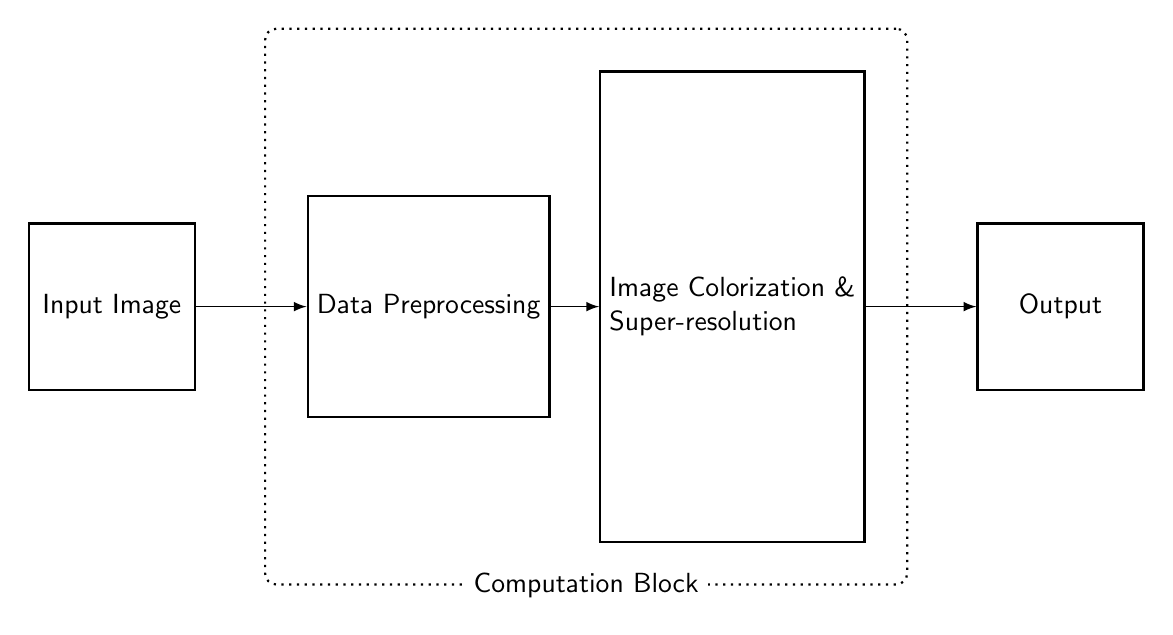
\begin{tikzpicture}[box/.style={draw,thick,minimum width=5em,minimum
    height=10em},arj/.style={semithick,-latex}]
  \begin{scope}[start chain=A going right,oc/.style={join=by arj,on chain},
    font=\sffamily,node distance=1.75em]
   \node(input)[box,minimum height=6em,minimum width=6em,oc]{Input Image};
   \node(data preprocessing)[box,minimum height=8em,oc][right=4em of input]{Data Preprocessing};
   \node(main computation)[box,minimum height=17em,oc]{
   \begin{varwidth}{10em}
      Image Colorization \& \\Super-resolution
    \end{varwidth}
    };
   \node[box,minimum height=6em,minimum width=6em,oc][right=4em of main computation]{Output};
   
   \node[draw, thick, dotted, rounded corners, inner xsep=1.5em, inner ysep=1.5em, fit=(data preprocessing) (main computation)] (box) {};
   \node[fill=white] at (box.south) {Computation Block};
  \end{scope}
  
%   \begin{scope}[shift = {{($(input.south)+(0cm, -2cm)$)}}, start chain=A going right, oc/.style={join=by arj, on chain},
%     font=\sffamily, node distance=1.75em]
%     \node[box,oc]{something};
%   \end{scope}
\end{tikzpicture}
\end{document}